\documentclass[tikz,border=5mm]{standalone}
\usepackage[utf8]{vietnam}
\usepackage{amsmath,amssymb}
\usepackage{tikz}
\usepackage{pgfplots}
\pgfplotsset{compat=1.18}
\usetikzlibrary{calc,shapes,backgrounds,arrows.meta,patterns,patterns.meta,angles,quotes}

\definecolor{slate}{RGB}{100,116,139}

\begin{document}
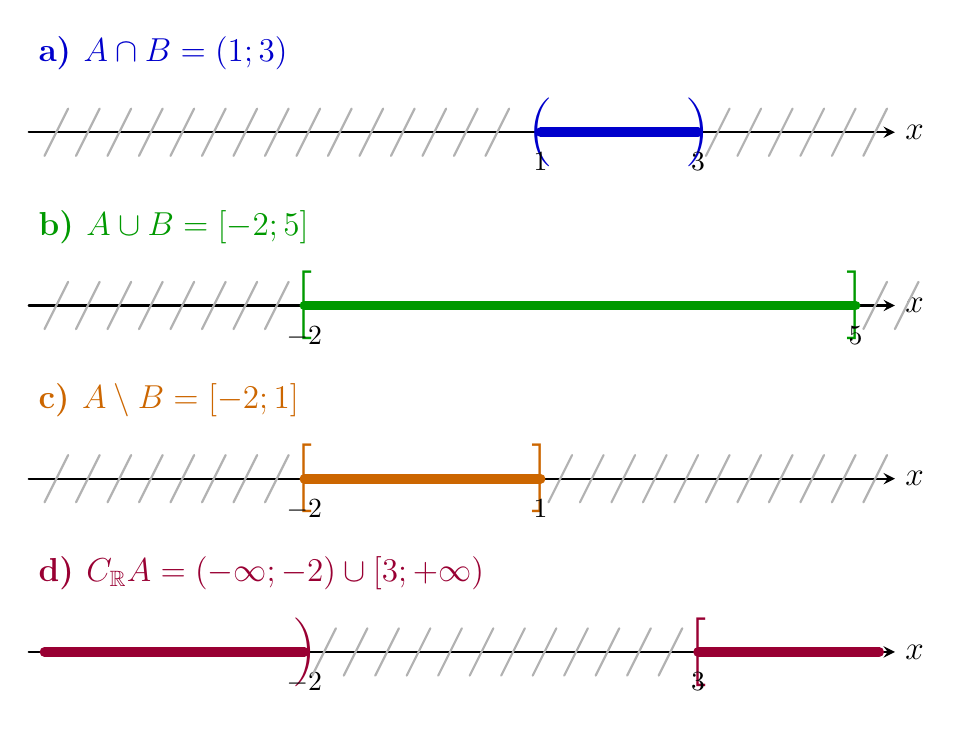
\begin{tikzpicture}[>=stealth,line join=round,line cap=round,font=\large]

  [every node/.style={font=\normalsize}]
  % 1. A \cap B = (1; 3)
  \node[anchor=west, font=\bfseries\large, text=blue!80!black] at (-5.5, 3.8) {a) $A \cap B = (1; 3)$};
  \draw[->, thick] (-5.5, 2.8) -- (5.5, 2.8) node[right] {$x$};
  \foreach \x in {-5.3,-4.9,...,0.7}
    \draw[gray!60, line width=0.8pt] (\x, 2.5) -- (\x+0.3, 3.1);
  \draw[line width=3.5pt, blue!80!black] (1, 2.8) -- (3, 2.8);
  \node[font=\Huge\bfseries, text=blue!80!black] at (1, 2.8) {$($};
  \node[below=4pt, text=black, font=\bfseries] at (1, 2.8) {$1$};
  \node[font=\Huge\bfseries, text=blue!80!black] at (3, 2.8) {$)$};
  \node[below=4pt, text=black, font=\bfseries] at (3, 2.8) {$3$};
  \foreach \x in {3.1,3.5,...,5.1}
    \draw[gray!60, line width=0.8pt] (\x, 2.5) -- (\x+0.3, 3.1);

  % 2. A \cup B = [-2; 5]
  \node[anchor=west, font=\bfseries\large, text=green!60!black] at (-5.5, 1.6) {b) $A \cup B = [-2; 5]$};
  \draw[->, thick] (-5.5, 0.6) -- (5.5, 0.6) node[right] {$x$};
  \foreach \x in {-5.3,-4.9,...,-2.3}
    \draw[gray!60, line width=0.8pt] (\x, 0.3) -- (\x+0.3, 0.9);
  \draw[line width=3.5pt, green!60!black] (-2, 0.6) -- (5, 0.6);
  \node[font=\Huge\bfseries, text=green!60!black] at (-2, 0.6) {$[$};
  \node[below=4pt, text=black, font=\bfseries] at (-2, 0.6) {$-2$};
  \node[font=\Huge\bfseries, text=green!60!black] at (5, 0.6) {$]$};
  \node[below=4pt, text=black, font=\bfseries] at (5, 0.6) {$5$};
  \foreach \x in {5.1,5.5,...,5.1}
    \draw[gray!60, line width=0.8pt] (\x, 0.3) -- (\x+0.3, 0.9);

  % 3. A \setminus B = [-2; 1]
  \node[anchor=west, font=\bfseries\large, text=orange!80!black] at (-5.5, -0.6) {c) $A \setminus B = [-2; 1]$};
  \draw[->, thick] (-5.5, -1.6) -- (5.5, -1.6) node[right] {$x$};
  \foreach \x in {-5.3,-4.9,...,-2.3}
    \draw[gray!60, line width=0.8pt] (\x, -1.9) -- (\x+0.3, -1.3);
  \draw[line width=3.5pt, orange!80!black] (-2, -1.6) -- (1, -1.6);
  \node[font=\Huge\bfseries, text=orange!80!black] at (-2, -1.6) {$[$};
  \node[below=4pt, text=black, font=\bfseries] at (-2, -1.6) {$-2$};
  \node[font=\Huge\bfseries, text=orange!80!black] at (1, -1.6) {$]$};
  \node[below=4pt, text=black, font=\bfseries] at (1, -1.6) {$1$};
  \foreach \x in {1.1,1.5,...,5.1}
    \draw[gray!60, line width=0.8pt] (\x, -1.9) -- (\x+0.3, -1.3);

  % 4. C_R A = (-\infty; -2) \cup [3; +\infty)
  \node[anchor=west, font=\bfseries\large, text=purple!80!black] at (-5.5, -2.8) {d) $C_{\mathbb{R}} A = (-\infty; -2) \cup [3; +\infty)$};
  \draw[->, thick] (-5.5, -3.8) -- (5.5, -3.8) node[right] {$x$};
  \draw[line width=3.5pt, purple!80!black] (-5.3, -3.8) -- (-2, -3.8);
  \node[font=\Huge\bfseries, text=purple!80!black] at (-2, -3.8) {$)$};
  \node[below=4pt, text=black, font=\bfseries] at (-2, -3.8) {$-2$};
  \foreach \x in {-1.9,-1.5,...,2.8}
    \draw[gray!60, line width=0.8pt] (\x, -4.1) -- (\x+0.3, -3.5);
  \draw[line width=3.5pt, purple!80!black] (3, -3.8) -- (5.3, -3.8);
  \node[font=\Huge\bfseries, text=purple!80!black] at (3, -3.8) {$[$};
  \node[below=4pt, text=black, font=\bfseries] at (3, -3.8) {$3$};

\end{tikzpicture}
\end{document}
